\section{Wire sagging}

	Easy to predict that the displacement of the wire invokes distortion an electric field (see figs~\ref{fig:elFieldCentered},\ref{fig:elField1mmShifted}) and drift path for electrons/ions inside the tube (see fig.\ref{fig:electron_ion_track} and Fig.\ref{fig:electron_ion_track_sag}). The RT-relation for track reconstruction directly depends on the wire position in the tube. So RT-relation loses it's previous symmetry (see next sections).
	
	\begin{figure}[h!]
		\centering
		\subfloat[wire in the center of the tube]{
			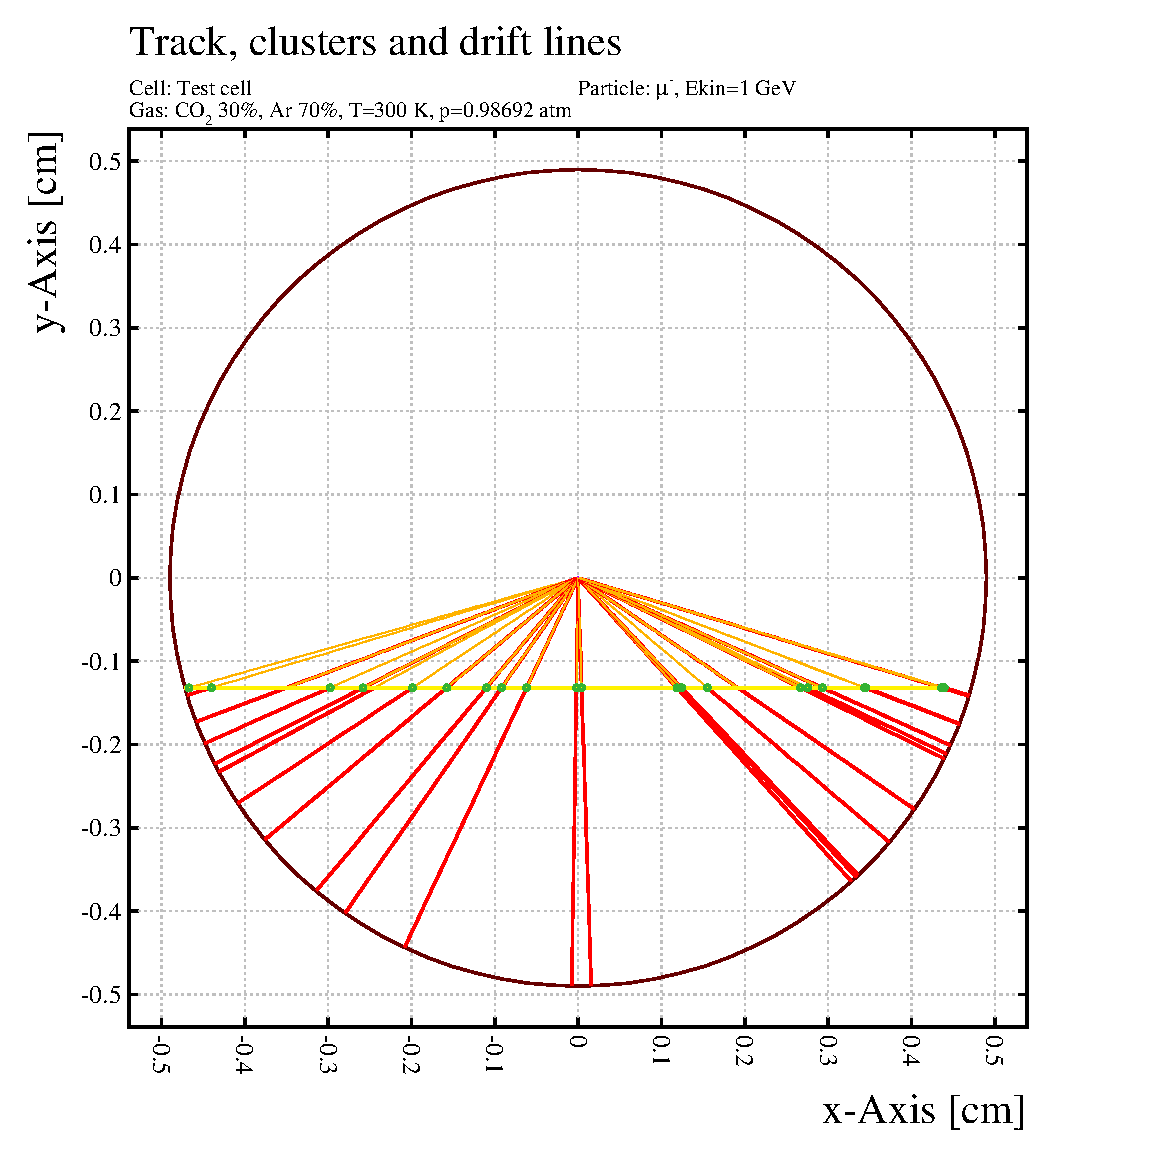
\includegraphics[width=0.45\textwidth]{sag/tracksAndClusters00Sag.eps} 
			\label{fig:electron_ion_track} }%
		\qquad
		\subfloat[sagging $1.5 mm$]{
			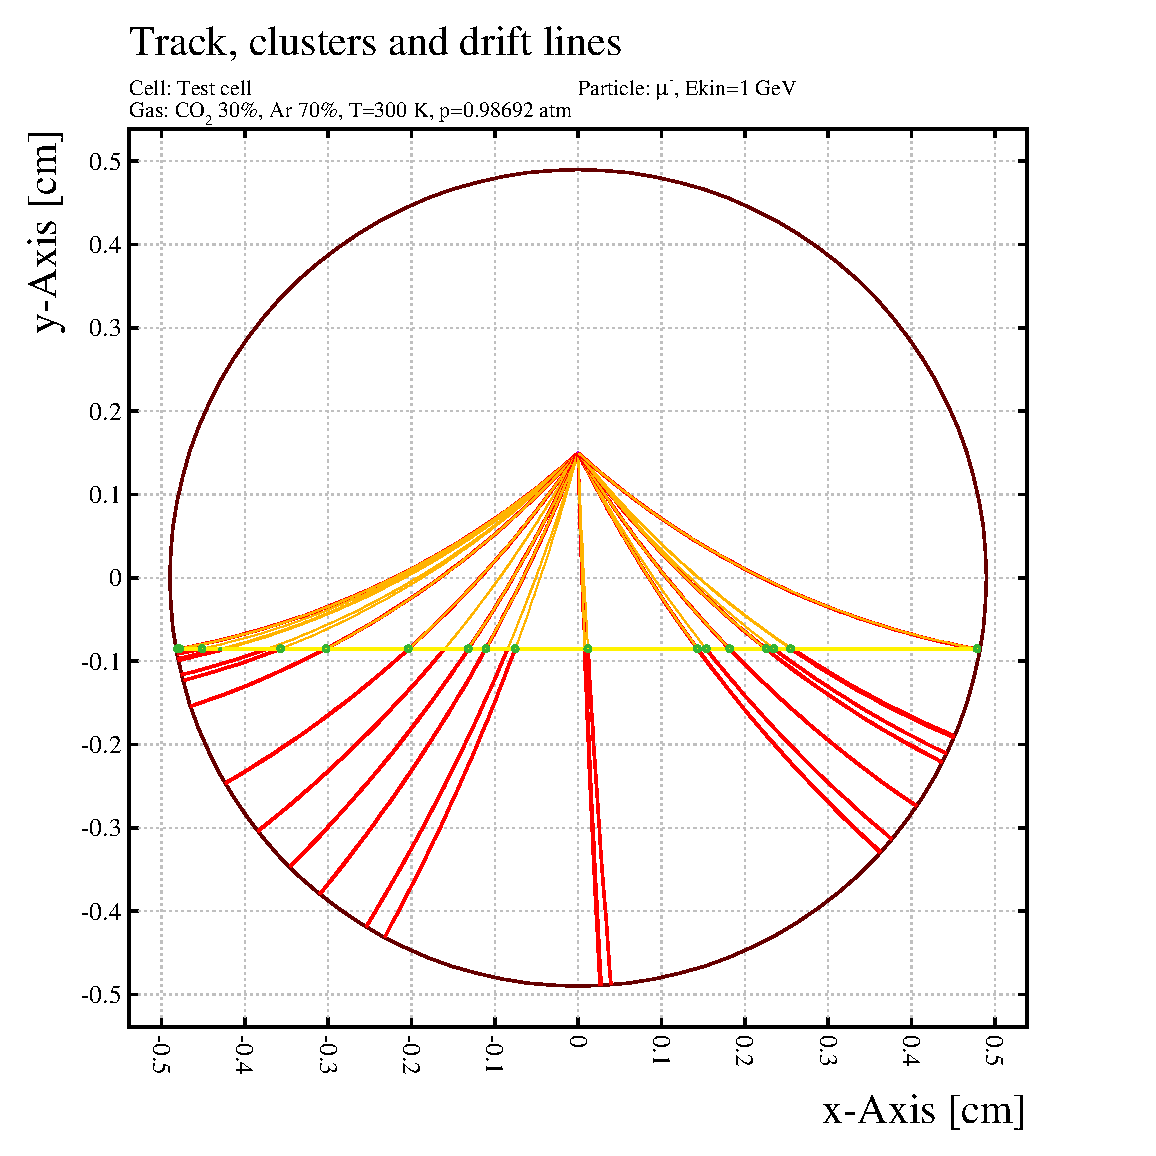
\includegraphics[width=0.45\textwidth]{sag/tracksAndClusters15Sag.eps} 
			\label{fig:electron_ion_track_sag} }%
		\caption{ An example of tracks from the on the tube for different position of the wire from GARFIELD simulations. Initial clusters marker by green. Drift lines for electrons marked by yellow, ions -- red lines.}	
	\end{figure}
	
	The direction of sagging is unpredictable when the wire is centered and the straw has vertical orientation. Impact of gravitation field into the wire does not make any effect in this state. But we can avoid this ambiguity by setting straws horizontally. This condition is necessary to make track reconstruction possible.
	Even when strung with a pulling force $T$ close to the breaking limit, wires in several metre long tubes will experience a gravitational sag that is large in comparison with the achievable accuracy of drift tubes.
	
	
	We estimate significant wire sagging(by comparison to the tube radius) because of wire attraction to the tube under affecting of gravitation and electric field force.
	
	You can see a profile of wire sagging of $5m$ length wire in $1cm$ diameter straw tube and 1750V voltage on the Fig.\ref{fig:sagProfile} calculated in GARFIELD software \cite{garfield}.
	
	\begin{figure}[h!]
	\centering
	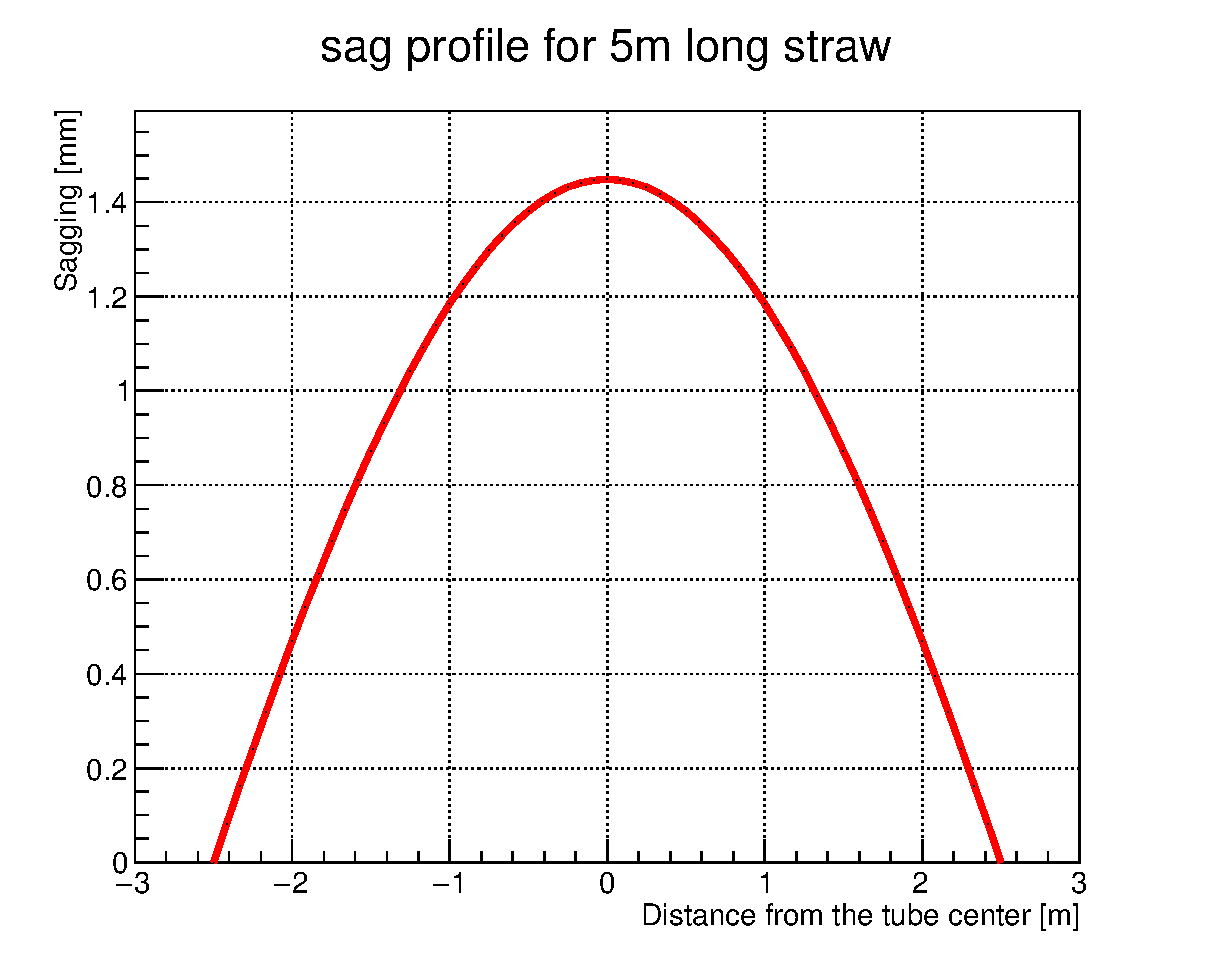
\includegraphics[width=0.7\textwidth]{sagProfileFit.eps}
	\caption{Wire sag profile under electric and gravitation field calculated in GARFIELD. All options for this straw system are described in table~\ref{table:straw_par}.}
	\label{fig:sagProfile}
	\end{figure}	
	
	The calibration of STRAW tube with sagged wire is more difficult by comparison to the mode without sagging. 
	
	Variation of wire tension, wire radius should be taken into account as high affect factor for sag value.
	
	\section{Sag estimation}
	\label{sec:sagEstimation}
	In this section we have to find out method for assessing sagging. This is key step that makes track reconstruction procedure possible.
	
	At first we have to think on data we can use for such kind of calculations. We can extract much useful information  from drift time distribution.
	
	The wire sags under electric and gravitation force. Therefore the sag value differs along the tube (Fig.\ref{fig:sagProfile}). But we can separate collected data for different position along the tube. STRAW tube detector consists of several parallel layers of tubes at some angle to each other. So we can easily fix longitudinal position (along the tube) for tracks that cross several crossed tubes (at least two). Collimation is also possible via scintillator triggering before and after STRAW tube.
	
	Lets say we can install our STRAW tube into homogeneous particle flow and save drift time distribution for some narrow section of the tube. These distributions are different from each other(see example on Fig.\ref{fig:DrftTimeDistr_00_09_comp}). The difference between diagrams increasing with sag difference. So it is good tools for sag calibration.
		
	\begin{figure}[h!]
	\centering
	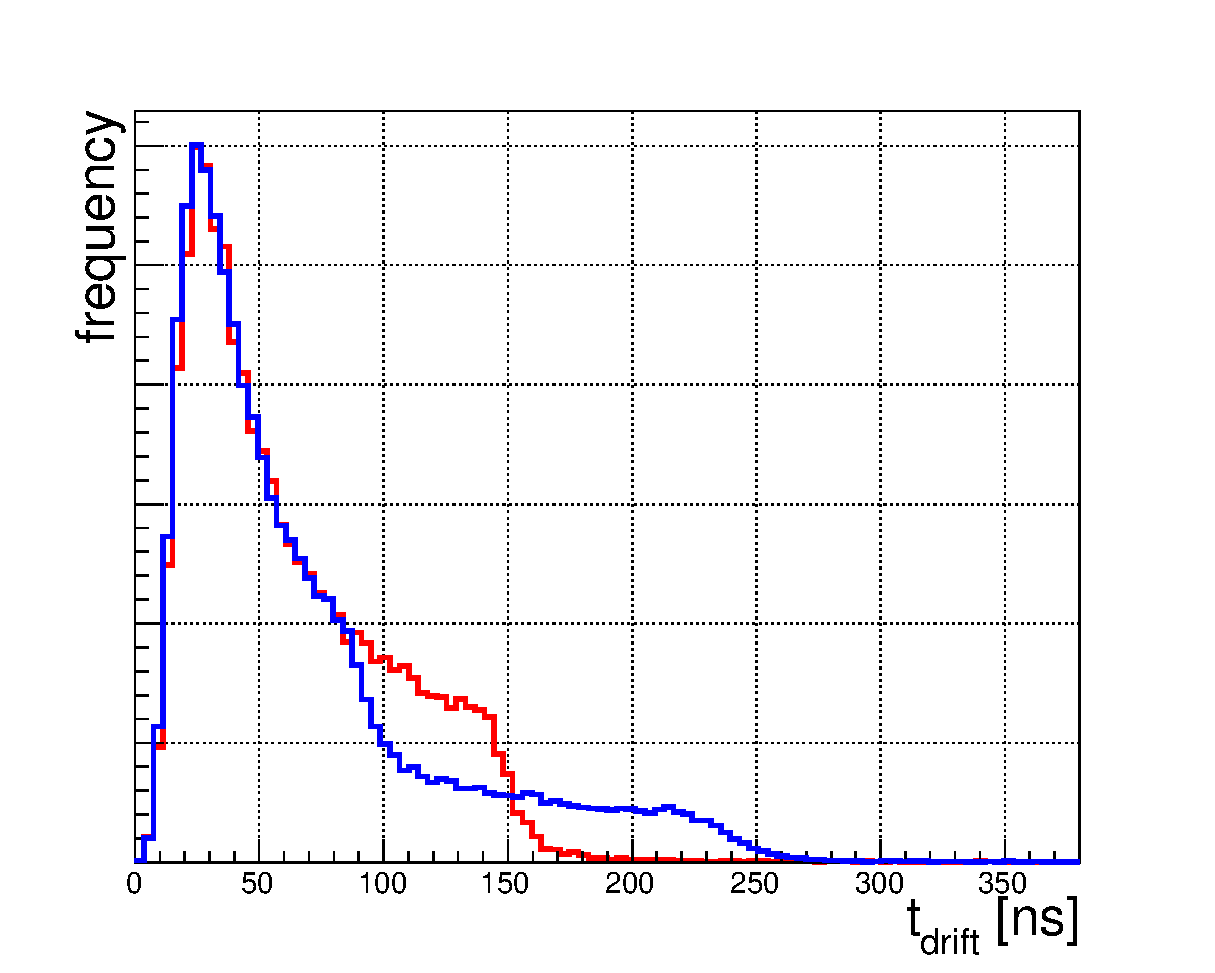
\includegraphics[width=0.8\textwidth]{00_09_driftTimeDistr}
	\caption{Drift time distribution for a homogeneous irradi-
ation with a centered wire (red) and for a wire offset of 0.9 mm (blue).}
	\label{fig:DrftTimeDistr_00_09_comp}	
	\end{figure}
	
	Then we have to bind each drift time distribution with appropriate sag value. This is part of laboratory work when sag profile measurements can be performed via optical method prior to the exposition.
	
	GARFIELD can handle only two-dimensional tasks. So every simulation in this article is plane - as shown in Fig.\ref{fig:electron_ion_track}.
	Distributions on Fig.\ref{fig:DrftTimeDistr_00_09_comp} contains GARFIELD simulations for tube with wire located at certain position (in terms of displacement from tube center).
	
	Lets say we have an equipment for scanning the tube to measure wire sagging profile. After profile measurements we divide our tube into sections.Wire position within separate section should be defined within desired precision
	
	So we need divide our tube on $57$ sections (see Fig.\ref{fig:tube_sectioning}) if maximum of wire offset (at the center of the tube) is equal to $1.45mm$ and desired precision is $50\mu m$.
	
	\begin{equation}
	N_{halftube} = \frac{1.45 mm}{50 \mu m} = 29;
	\label{eq:tube_sectioning}
	\end{equation}
	
	\begin{figure}[h!]
	\centering
	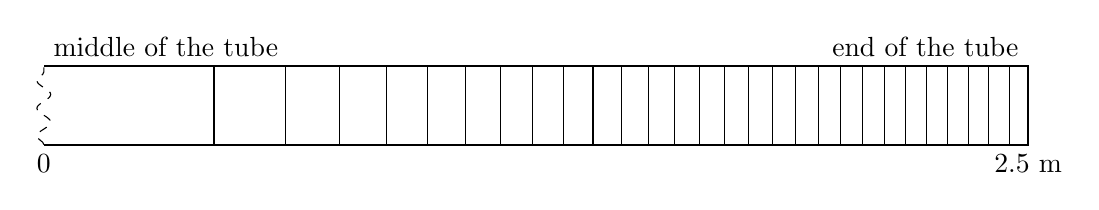
\begin{tikzpicture}[xscale=0.05,yscale=1]
	
	\tikzset{snake it/.style={decorate, decoration=snake}}
	\draw[snake it,dashed] (0,0) -- (0,1);
	
	\draw[thick] (0,0) -- (250,0) -- (250,1) -- (0,1);
	\draw[] (43.2339,0) -- (43.2339,1) -- 
	(61.2704,1) -- (61.2704,0) -- 
	(75.2004,0) -- (75.2004,1) -- 
	(87.0213,1) -- (87.0213,0) -- 
	(97.5056,0) -- (97.5056,1) -- 
	(107.049,1) -- (107.049,0) -- 
	(115.885,0) -- (115.885,1) -- 
	(115.885,1) -- (115.885,0) -- 
	(124.169,0) -- (124.169,1) -- 
	(132.005,1) -- (132.005,0) -- 
	(139.472,0) -- (139.472,1) -- 
	(146.627,1) -- (146.627,0) -- 
	(153.516,0) -- (153.516,1) -- 
	(160.176,1) -- (160.176,0) -- 
	(166.636,0) -- (166.636,1) -- 
	(172.921,1) -- (172.921,0) -- 
	(179.05,0) -- (179.05,1) -- 
	(185.043,1) -- (185.043,0) -- 
	(190.913,0) -- (190.913,1) -- 
	(196.674,1) -- (196.674,0) -- 
	(202.338,0) -- (202.338,1) -- 
	(207.915,1) -- (207.915,0) -- 
	(213.414,0) -- (213.414,1) -- 
	(218.844,1) -- (218.844,0) -- 
	(224.212,0) -- (224.212,1) -- 
	(229.527,1) -- (229.527,0) -- 
	(234.793,0) -- (234.793,1) -- 
	(240.018,1) -- (240.018,0) -- 
	(245.207,0) -- (245.207,1);
	
	\node[below] at (0,0) {0};
	\node[below] at (250,0) {2.5 m};
	\node[above right] at (0,1) {middle of the tube};
	\node[above left] at (250,1) {end of the tube};
	
	\end{tikzpicture} 
	\caption{Tube sectioning. Sag value at the tube center is $1.45mm$. Difference of wire sag value from section to section is $50\mu m$}
	\label{fig:tube_sectioning}
	\end{figure}
	
	Then we need an exposition of sufficient number of events for every of sections(at least 50k events). There can be troubles time of exposition time because square of sections at the end of the tube is quite small. So the time of exposition of distant sections will be inversely much longer.
	
	The next step is to find dependence of dt-distribution shape with wire offset. The point that we can evaluate matching between histograms via $\chi^2$  criteria. As we can see in the figure~\ref{fig:chi2for07} the comparison of  $\chi^2$ has smooth dependence across increasing of wire offset for high statistic histograms.
		
	First steps for sag estimation are:
	\begin{enumerate}
	\item measure wire sag profile via optical method;	
	\item make a sectioning of tube due to wire sag profile;
	\item collect enough amount of events for every of dt-distribution and save this {\it core} distribution for further comparisons.
	\item measure dt-distribution of tube section that is subject of study and and adjacent area.
	\item calculate $\chi^2$ criteria for this current dt-distribution with each of core distribution.
	\item correlate found values of wire displacement relatively to the adjacent sections or by fitting of whole wire profile points.
	\end{enumerate}

	\subsection{Finding most probable value of wire displacement for certain point of the tube}
	
	\subsection{Raw method}
	The simplest method to find $S$ is to equate it to the corresponding value of best matched core DT-histogram.
	
	On the figure \ref{fig:chi_063_5k}  you can see distribution of such kind of reconstruction. Even for 5k events td-distribution in this case the precision can be quite high($\sim 50 \mu m$). This method limited by core DT-diagram stepping.
	
	\begin{figure}[h!]
		\centering
		\subfloat[Series of $\chi^2$ of comparison $0.7 mm$ sag core td-distribution with each each of core histograms. 14 core histograms for sag diapason $0\dots 1.3 mm$ with step of $100\mu m$]{
			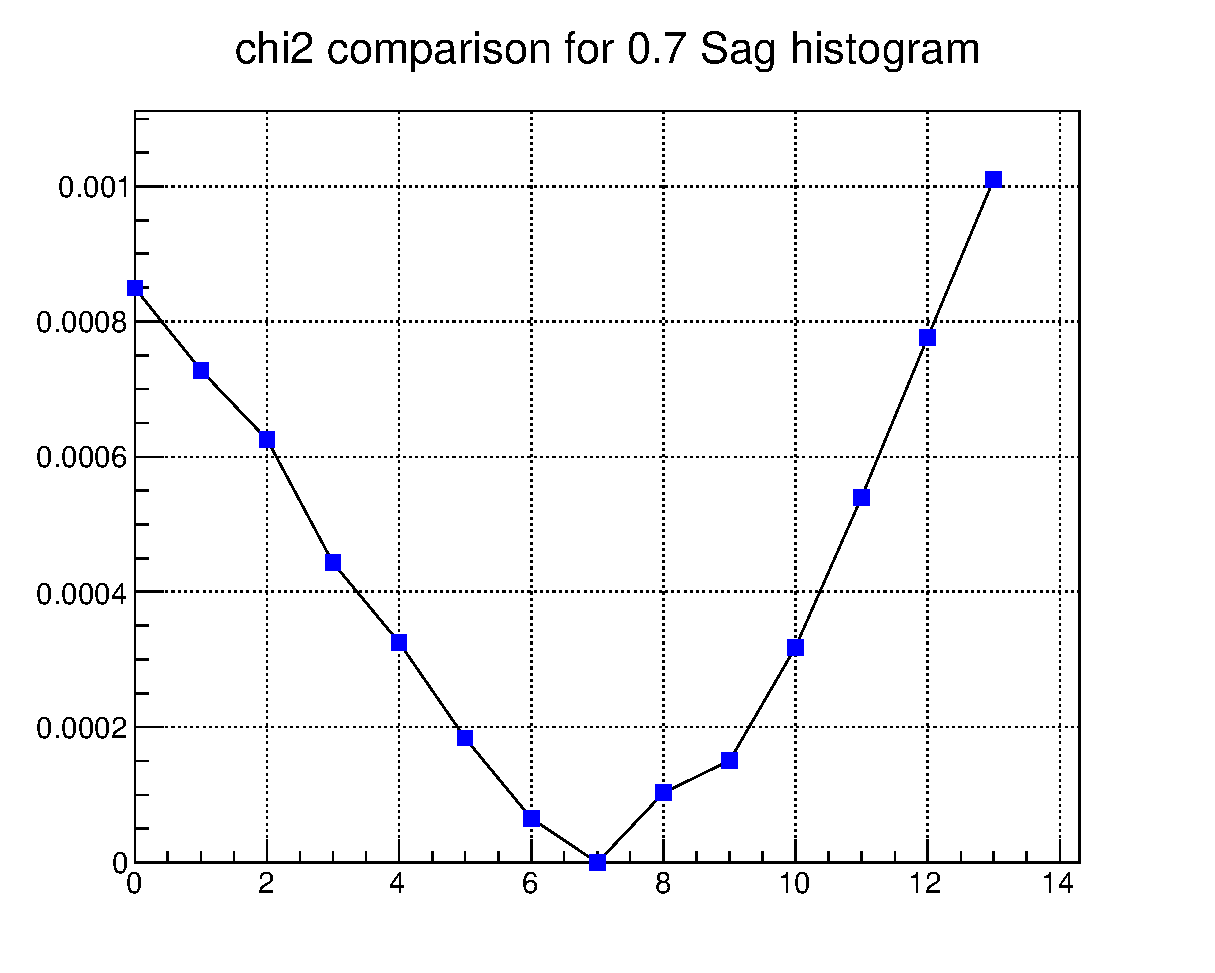
\includegraphics[width=0.45\textwidth]{chi2_07} 
			\label{fig:chi2for07} }%
		\qquad
		\subfloat[ Distribution of wire offset reconstruction from 180 series 5k events each. 50k events for $core$ template histograms. True bias is $0.63 mm$. 1 bin = 0.1 mm.]{
			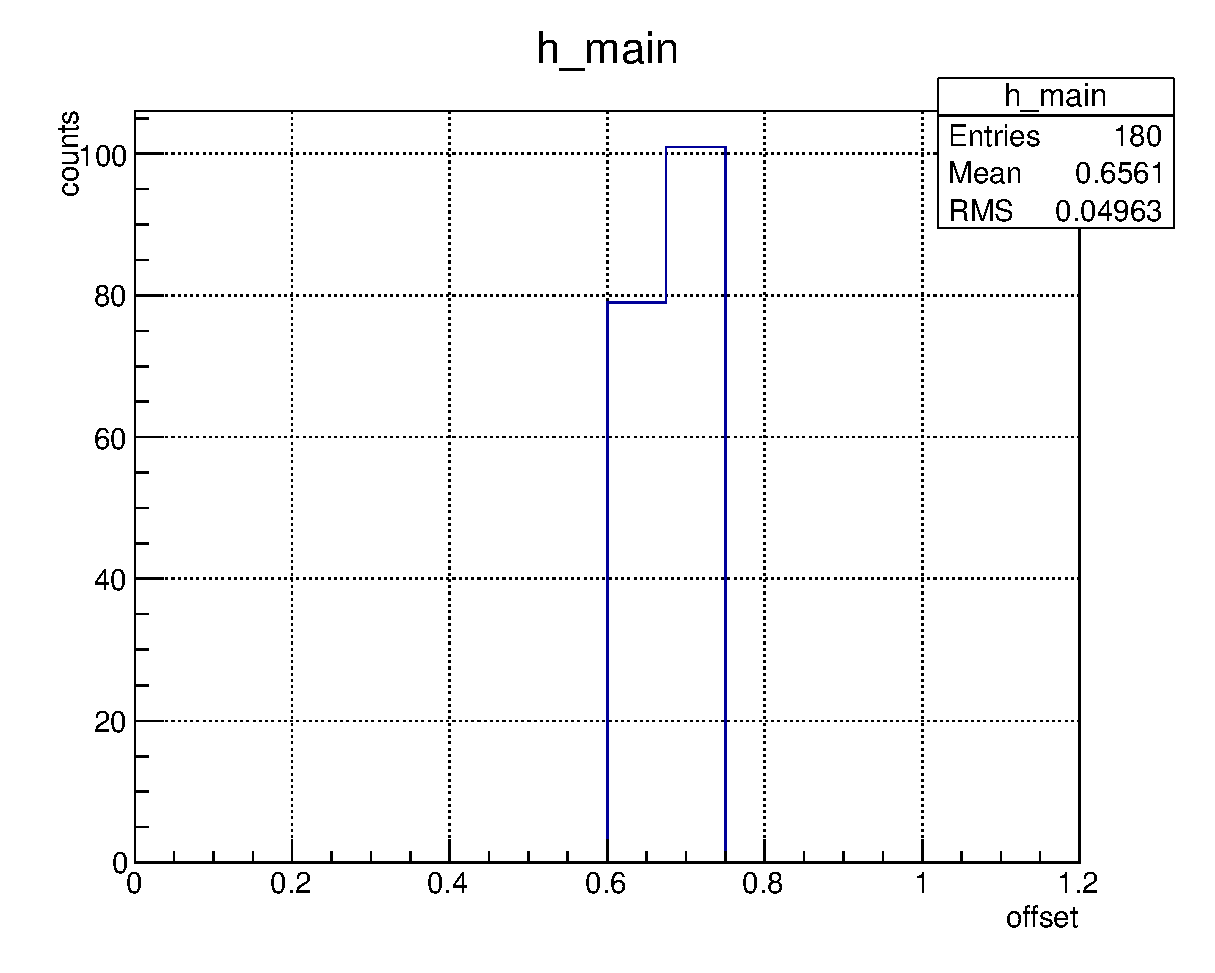
\includegraphics[width=0.45\textwidth]{chi_063_5k} 
			\label{fig:chi_063_5k} }%
		\caption{Wire position(displacement) reconstruction}			
	\end{figure}	
	
%	If we compare dt-distribution for $0.7mm$ displaced wire with each of core dt-distribution you will notice best matching with core histogram for the same wire displacement(see fig see fig~\ref{fig:chi2for07}).
	

	\subsection{"Minimum of $\chi^2$ as linear approximation"}
%	But what is most probable value of wire displacement $S$ in this case? Probably somewhere between them. So can we go in more clever way to reach better result? Probably yes.
	
	If dependence of $\chi^2$ criteria of wire displacement $S$ for near to the true position region is linear(that certainly is not a true, but as first approximation) than we can easily find this intermediate value of wire displacement.
	
	There we proceed in two steps. The first is raw estimation of wire displacement as in above mentioned method.
	
	For the second step we need to know some additional estimations.	The first question is how small can be  $\chi^2$ it our case? Lets fix statistic on 50k events for one DT-distribution. This value should a bit depend for different $S$. But for now lets consider that it is a constant value. From the Fig.\ref{fig:chi2Shelf} you can see distribution of $\chi^2$ from comparison of 20 DT-distribution\footnote{pair comparison give us $C_{20}^2 = \frac{20!}{2!18!}=190$ different combinations}  for $S=0.7mm$. Mean value + RMS of distribution is $ 5.3*10^{-5}$. So if some of the $\chi^2$ is higher than this threshold than we go for second stage.
	
	
	\begin{figure}[h!]
		\centering
		\subfloat[$\chi^2$ distribution of comparison of 20 DT-distributions diagrams each other($C_{20}^2 = 190$ combinations)]{
			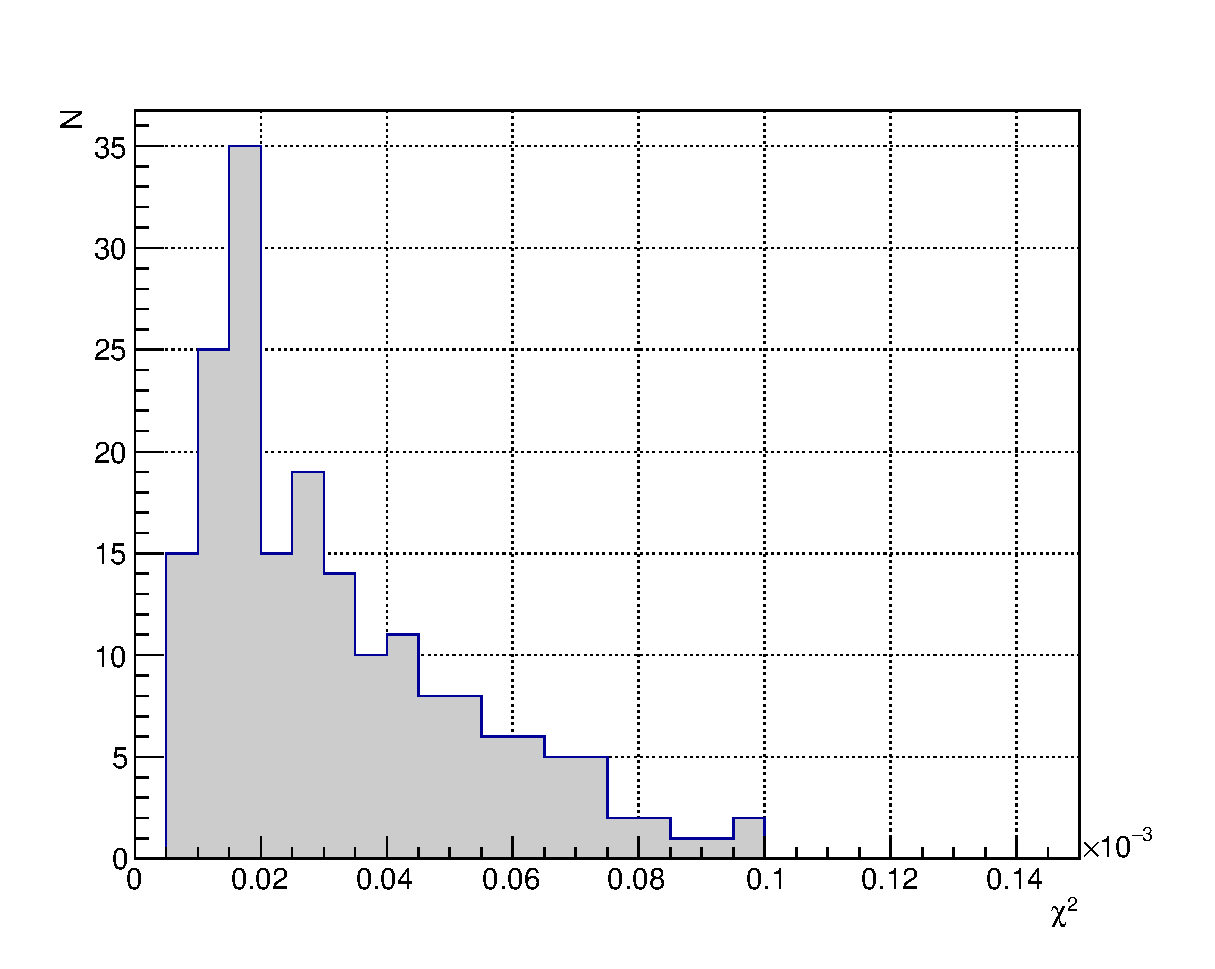
\includegraphics[width=0.45\textwidth]{chi2Shelf} 
			\label{fig:chi2Shelf} }%
		\qquad
		\subfloat[$\chi^2$ distribution of comparison DT-distribution histograms $0.6 mm$ S vs $0.7 mm$ ]{
			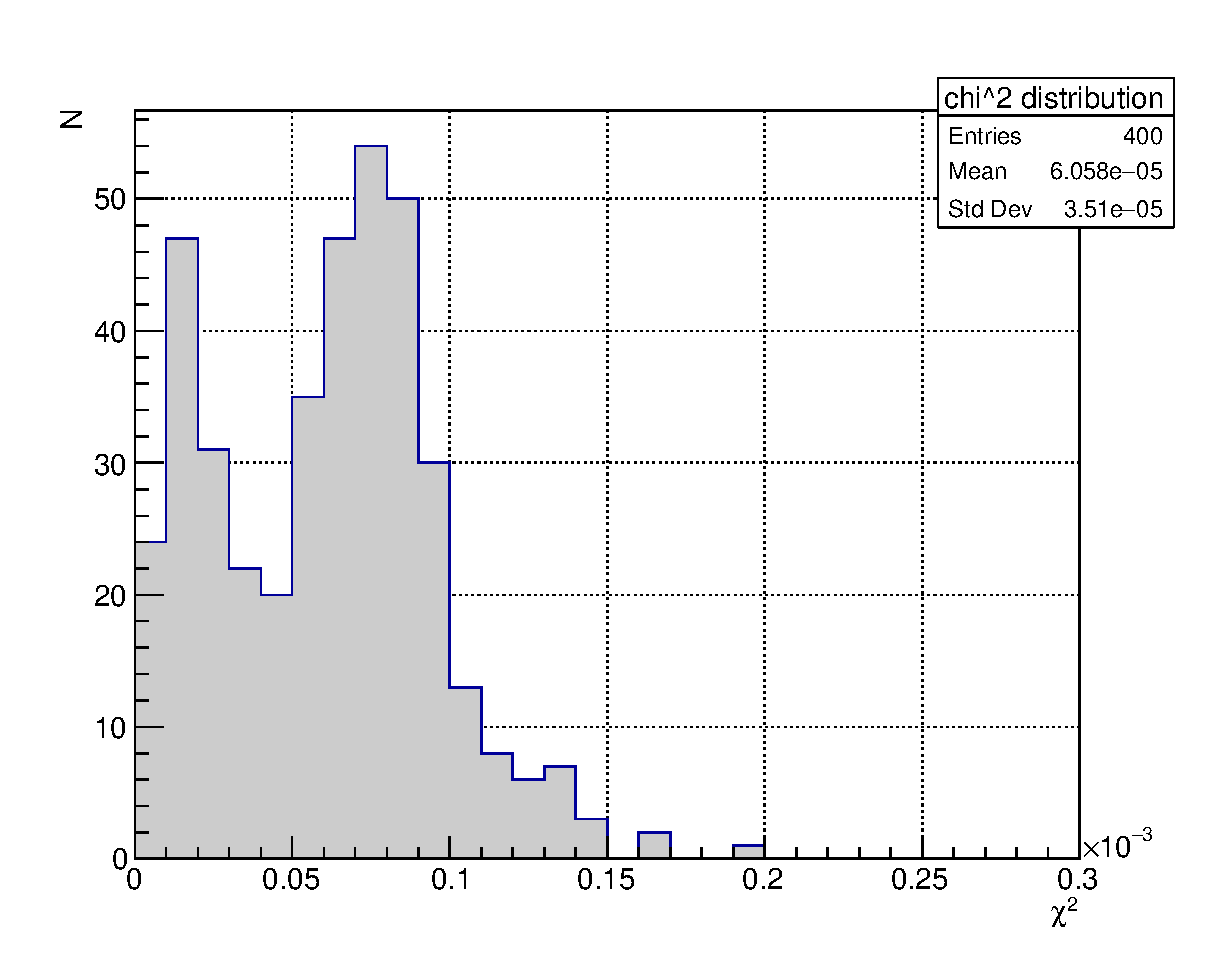
\includegraphics[width=0.45\textwidth]{06_07_chi_stat} 
			\label{fig:06_07_chi_stat} }%
		\caption{Comparison of $\chi^2$ distributions for self-comparison of DT-distribution diagram.} 
	\end{figure}	
	
	On the Fig.\ref{fig:chi_063_5k} you can see distribution of wire sag calculation for 180 histograms with 5k events statistic. Precision in this case  $\sim 50\mu$. The algorithm of sag estimation is pretty simple: wire offset value is equal to the offset  of best matched  $core$ histogram.

	After we know sag value at some points of the tube or every where we can make one awesome collective analysis. The smoothing of wire offset value along the tube will give to us much more precision results.  
	
	From the Fig.\ref{fig:06_07_chi_stat} the distribution of $\chi^2$ for adjacent point have narrower distribution by comparison to "self-comparison" $\chi^2$ distribution. Therefore calculation of $S$ from analyse of consecutive smallest $\chi^2$ values can improve precision.
	Need to say that collective approach to this task also can improve precision of $S$ finding. 
	
	
	\subsection{Practical measurements of DT-distribution}
	
	We need second detector that can measure position of muon that hit STRAW tube. It can be Si strip sensor based detector or detector based on  scintillation with the same destination.
	
	Each kind of detector have it's own advantages and disadvantages. The potential cell unit (strip of pixel) of Si detector will be smaller than in scintilator but also is match expensive. At the current stage we deal with $1cm$ diameter tubes. So scintilator is primal target. But it can shift to the Si sensors if scintilators will not provide satisfied precision.
	
	Preliminary chem of DT-measurements you can see on the picture Fig.\ref{fig:DT-mesure-layout}
	
	\begin{figure}[h!]
	\centering
	\begin{tikzpicture}
	
	\tikzset{snake it/.style={decorate, decoration=snake}}
	
	\draw (-1,0) -- (-1,10);
	\draw ( 1,0) -- ( 1,10);
	\draw (0,0) ellipse (1 and .3);
	\draw (0,10) ellipse (1 and .3);
	
	\draw (-5,0) -- (-6,0);
	\draw (-5,.5) -- (-6,.5);
	\draw (-5,1) -- (-6,1);
	\draw (-5,1.5) -- (-6,1.5);
	\draw (-5,2) -- (-6,2);
	\draw (-5,2.5) -- (-6,2.5);
	\draw (-5,3) -- (-6,3);
	\draw (-5,3.5) -- (-6,3.5);
	\draw (-5,4) -- (-6,4);
	\draw (-5,4.5) -- (-6,4.5);
	\draw (-5,5) -- (-6,5);
	\draw (-5,5.5) -- (-6,5.5);
	\draw (-5,6) -- (-6,6);
	\draw (-5,6.5) -- (-6,6.5);
	\draw (-5,7) -- (-6,7);
	\draw (-5,7.5) -- (-6,7.5);
	\draw (-5,8) -- (-6,8);
	\draw (-5,8.5) -- (-6,8.5);
	\draw (-5,9) -- (-6,9);
	\draw (-5,9.5) -- (-6,9.5);
	\draw (-5,10) -- (-6,10);
	
	\draw (-5,0) -- (-5,10);
	\draw (-6,0) -- (-6,10);

	\draw (5,0) -- (6,0);
	\draw (5,.5) -- (6,.5);
	\draw (5,1) -- (6,1);
	\draw (5,1.5) -- (6,1.5);
	\draw (5,2) -- (6,2);
	\draw (5,2.5) -- (6,2.5);
	\draw (5,3) -- (6,3);
	\draw (5,3.5) -- (6,3.5);
	\draw (5,4) -- (6,4);
	\draw (5,4.5) -- (6,4.5);
	\draw (5,5) -- (6,5);
	\draw (5,5.5) -- (6,5.5);
	\draw (5,6) -- (6,6);
	\draw (5,6.5) -- (6,6.5);
	\draw (5,7) -- (6,7);
	\draw (5,7.5) -- (6,7.5);
	\draw (5,8) -- (6,8);
	\draw (5,8.5) -- (6,8.5);
	\draw (5,9) -- (6,9);
	\draw (5,9.5) -- (6,9.5);
	\draw (5,10) -- (6,10);
	
	\draw (5,0) -- (5,10);
	\draw (6,0) -- (6,10);
	
	\node [below] at (5,0) {detector 2};
	\node [below] at (-5,0) {detector 1};
	\node [] at (0,-1) {STRAW tube};


	\draw[ultra thick,->] (-10,7.5) -- (-6.5,7.5);
	\draw[ultra thick,->] (-10,7) -- (-6.5,7);
	\draw[ultra thick,->] (-10,6.5) -- (-6.5,6.5);
	\draw[ultra thick,->] (-10,6) -- (-6.5,6);
	\draw[ultra thick,->] (-10,5.5) -- (-6.5,5.5);
	\draw[ultra thick,->] (-10,5) -- (-6.5,5);
	
	\node at (-8,8) {muon flow};
	
	\draw[thick] (-8,3) ellipse (0.3 and 0.3);
	
	\draw[thick] (-8-0.2, 3-0.2) --(-8 +0.2, 3+0.2);
	\draw[thick] (-8-0.2, 3+0.2) --(-8 +0.2, 3-0.2);

	\node[] at (-8.5,3) {$\vec{g}$};
		
	\end{tikzpicture} 
	\caption{principal layout of measurement of core DT-distribution histogram}
	\label{fig:DT-mesure-layout}
	\end{figure}	
	
	In this method detector before tube (D1) and detector placed after the tube(D2) in total should provide sufficient precision for track reconstruction to be able distinguish tracks for different section of the tube (approximately as shown on the Fig. \ref{fig:tube_sectioning}). Muon flow should be homogeneous and so D1 and D2 also should cover full acceptance of the tube.
	
	The profile of the wire sagging can be measured by optical method. Walls of the tube is very thin, so it can be simplest way to get sag profile.
	